\section{Evaluation}
\label{sec:eval}

In this section, we introduce the datasets used in our experiments and the experimental setup. We design two experiments, 
\textbf{general length control} and \textbf{zero-shot length control},
to compare our proposed approach with baselines.
General length control experiment trains and tests the models on complete original dataset.
Zero-shot length control experiment trains the model on training set removing the samples within a length range,
and tests the model on the samples within this length range.
%For zero-shot length control experiment,
%we first set a length range $(0, len]$. 
%Then we train the models on training data removing the samples with lengths in $(0, len]$, and tests the models on samples in test data with lengths in $(0, len]$ .

\subsection{Dataset}
We use 2 popular datasets in abstractive summarization in our experiment.
\textbf{CNN/Daily Mail Dataset}
(CNNDM)~\cite{HermannKGEKSB15}
\footnote{https://cs.nyu.edu/˜kcho/DMQA/},
consists of pairs of a single source document and a multi-sentence summary.
The dataset includes 286,817 training pairs,
13,368 validation pairs and 11,487 test pairs.
%\tabref{table:cnn} shows an example pair from training data.
%We follow the same pre-processing step used by \citep{SeeLM17},
%and fill in the blanks with answer named entities.
\textbf{XSUM Dataset}
%\footnote{https://github.com/EdinburghNLP/XSum} 
\cite{XSUM} is composed of paired articles and single-sentence summaries. 
The number of samples in training/validation/test sets are 204,045/11,332/11,334.

The length distribution of these two datasets are shown in \tabref{tab:lendis}. 
We follow~\citet{LiuLZ18} and \citet{Proto20}
to segment the dataset by different length ranges.
As the lengths of summaries in XSUM are shorter, 
the summary length of XSUM is divided into 3 length ranges.
For general length control experiments,
we take all samples of CNNDM and XSUM for training and test, as shown in \tabref{tab:lendis} (a).
For \textbf{zero-shot experiments}, 
we remove the samples with short summaries within a length range $R$ from training and validation set, and take these samples as test set.
To make sure the number of samples in test set comparable,
the $R$ for CNNDM and XSUM is $(0,30]$ and $(0,10]$, containing $488$ and $176$ samples respectively.
\cut{%%%%
\begin{table}[th]
	\scriptsize
	\centering
		\begin{tabular}{|c|r|rrr|rrr|}
			\hline
			\multirow{2}{*}{\bf Data} & \multirow{2}{*}{\bf Length} & \multicolumn{3}{c|}{General} & \multicolumn{3}{c|}{Zero-shot} \\ \cline{3-8}
			& & \bf Train & \bf Val & \bf Test & \bf Train & \bf Val & \bf Test \\ 
			\hline
			\multirow{7}{*}{CNNDM} 
			&$(0,10]$ & 421 &1 &1 &-&-&1\\
			& $(10,30]$ & 20,429&573 & 487 & & &\\
			& $(30,50]$ & 114,521 &4,255&4,144 & & &\\
			& $(50,70]$& 101,461 & 4,746 &4,380 & & &\\
			& $(70,90]$ & 31,470 & 2,321 & 1,509& & &\\
			& $(90,+\infty)$ & 18,925&1,472 &969 & & &\\
			\cline{2-8}
			&Total &287,228&13,369&11,491 & & &\\
			\hline
			\multirow{4}{*}{XSUM} 
			&$(0,10]$ & 3,049 & 167 & 176 & & &\\
			& $(10,30]$ & 193,237 & 10,732 & 10,729 & & &\\
			& $(30,+\infty)$ & 77,60 & 433 & 429 & & &\\
			\cline{2-8}
			&Total &204,046&11,332&11,334& & &\\
			\hline
		\end{tabular}
		\caption{The number of summaries within different length ranges.}
	\label{tab:lendis}
\end{table}
}%%%%

\begin{table}[th]
	\scriptsize
	\centering
%	\subtable[\bf General Length control]{
	\begin{tabular}{|c|r|rrr|}
		\hline
		\bf Data& \bf Length& \bf Train & \bf Val & \bf Test \\ 
		\hline
		\multirow{7}{*}{CNNDM} 
		&$(0,10]$ & 421 &1 &1 \\
		& $(10,30]$ & 20,429&573 & 487\\
		& $(30,50]$ & 114,521 &4,255&4,144 \\
		& $(50,70]$& 101,461 & 4,746 &4,380 \\
		& $(70,90]$ & 31,470 & 2,321 & 1,509\\
		& $(90,+\infty)$ & 18,925&1,472 &969 \\
		   		\cline{2-5}
		&Total &287,228&13,369&11,491 \\
	    \hline
	    \multirow{4}{*}{XSUM} 
	    &$(0,10]$ & 3,049 & 167 & 176 \\
	    & $(10,30]$ & 193,237 & 10,732 & 10,729 \\
	    & $(30,+\infty)$ & 77,60 & 433 & 429 \\
	       		\cline{2-5}
	    &Total &204,046&11,332&11,334\\
		\hline
	\end{tabular}
%}
%   \qquad
%   \subtable[{\bf Zero-shot Length control}]{
%   	\begin{tabular}{|c|r|rrr|}
 %  		\hline
%   		\bf Data& \bf Length & \bf Train & \bf Val & \bf Test \\ 
%   		\hline
%   		\multirow{7}{*}{CNNDM} 
%   		&$(0,10]$ & - &- &1 \\
%   		& $(10,30]$ & -&- & 487\\
%   		& $(30,50]$ & 114,521 &4,255&- \\
%   		& $(50,70]$& 101,461 & 4,746 &- \\
%   		& $(70,90]$ & 31,470 & 2,321 & -\\
%   		& $(90,+\infty)$ & 18,925&1,472 &- \\
%   		\cline{2-5}
%   		&Total &266,378&12,795&488 \\
%   		\hline
%   		\multirow{4}{*}{XSUM} 
%   		&$(0,10]$ & - & - & 176 \\
%   		& $(10,30]$ & 193,237 & 10,732 & - \\
 %  		& $(30,+\infty)$ & 77,60 & 433 & - \\
 %  		\cline{2-5}
 %  		&Total &200,997&11,165&176 \\
 %  		\hline
 %  	\end{tabular}
 %  }
	\caption{The number of summaries within different length ranges.}
	\label{tab:lendis}
\end{table}

\subsection{Baselines}
We take the length-controllable models with good preformance as the baselines, which are listed in \tabref{tab:baselines}.

\begin{table}[th]
	\scriptsize
	\centering
	\begin{tabular}{|m{1.5cm}<{\raggedleft}|p{5.6cm}|}
		\hline
		\textbf{Abbrev.} & \textbf{Description} \\ 
		\hline
		\multicolumn{2}{|c|}{\bf Abstractive summarization models} \\
		\hline
		PG & Pointer Generator.~\cite{SeeLM17} \\
		\hline
		BART & \tabincell{l}{Pretrained transformer seq2seq model.~\cite{BART19}}\\
		\hline
		\multicolumn{2}{|c|}{\bf Previous length-controllable models} \\
		\hline
		%Max & Insert $eos$ at the desired length during decoding at test.\\
		%\hline
		Exact & \tabincell{l}{Ignore $eos$ before generated summary within the desired \\ length and insert $eos$ at the desired length.} \\
		\hline 
		LenEmb & Input remaining length embeddings.~\cite{KikuchiNSTO16} \\
		\hline
		LC & Take desired length as input.~\cite{LiuLZ18}\\
		\hline
		GOLC & Apply length-aware loss.~\cite{GOLC19} \\
		\hline
		LenAtten &Add length attention unit.~\cite{lenatten21} \\
		\hline
		Prot & Extract prototype summary.~\cite{Proto20}\\
		\hline
	\end{tabular}
	\caption{The abbreviation and description of methods.}
	\label{tab:baselines}
\end{table}

In the experiments, we take BART as basic model,
because BART is one of the SOTA models in abstractive summarization and can be 
implemented on less memory and training time~\cite{analysis20}. our LAAM and LAAM
with pretraining (PtLAAM)
are implemented on top of our implementation of BART,
\footnote{In rest of this paper, LAAM refers to the BART using LAAM as cross-attention, for simplicity.}
 hence their results
are directly comparable. Exact is not a standalone model but is used in the decoder
of any seq2seq models to produce summary of exact lengths.  

All results on XSUM except for PG, and BART/LAAM related results
on CNNDM are produced by our own implementations of the respective models. All other results
are copied from the original publications. 

\subsection{Experimental Setup}
In our experiments, according to the length distributions of the summaries 
in CNNDM and XSUM~\tabref{tab:lendis}, 
we set the discrete bins $B$ of summary length ranges in \secref{sec:lbd} for CNNDM and XSUM.
The $B$ of CNNDM is $B_{c}=\left\{(0,10],(10,30],...,(90, +\infty)\right\}$ and that of XSUM is $B_{x}=\left\{(0,10],(10,30],(30, +\infty)\right\}$. 
During training and test,
we set the lengths of gold summaries as desired lengths and take them as input for length-controllable approaches.

Following~\citet{BART19},
we train our model based on  {\em bart.large} with
$lr=3e$-$05$ and warmup $=500$.
we set the dropout as $0.1$ and momentum as $0.99$.
We terminate the training process when the learning rate drops below $10e$-$5$. 
At test time, the batch size is $32$. 
We set beam size as $4$ for CNNDM and $6$ for XSUM in the testing step.
We train and test our models on one RTX 2080Ti GPU with 11G RAM. 

%In our experiment, we use the general ROUGE evaluation tool {\em files2rouge} in summarization tasks~\cite{BART19}.
%We set beam size as $4$ for the beam search algorithm in the testing step.

As the encoder-decoder models stop decoding by generating $eos$. 
To evaluate the ability of the models to control length,
we set the minimum length ($minlen$) equaling $0$ and maximum length ($maxlen$) equaling $200$ in generation parameters, covering the lengths of most reference summaries.
This is to make sure that the $eos$ is generated by models but not be designated by users.
%Thus, we set $minlen=0$ and $maxlen=200$ during test,
%which covers the lengths of most reference summaries.

%in the purpose of the other two versions is to enable fair comparison of the summaries in terms of their content given that the summaries are of equal length. 

\subsection{Evaluation metrics}
The evaluation metrics in our experiments are as follows:
\begin{enumerate}
\item \textit{ROUGE} scores (F1 score) include  ROUGE-1(R-1), ROUGE-2(R-2) and
ROUGE-L(R-L)~\cite{rouge}.
%ROUGE-2 is the most popular metric for summarization.

\item \textit{Variance} (Var) of the summary lengths against
the desired length $len$:
%The variance is computed as following:
\begin{equation}
var = 0.001 * \frac{1}{n}\sum_{i=0}^{n} |l_i - len|^2, 
\end{equation}
where $n$ is the number of pairs in dataset, and $l_i$ is the length of generated summary $i$. 
We use the variance to evaluate the
ability of exact control of the output length.

\item \textit{Human Evaluation.}
We randomly select 50 samples from CNNDM and 50 samples from XSUM.
We ask two human annotators
who are native or proficient English speakers to score 
the generated summaries comprehensively considering the consistency with the source document and informativeness,
i.e., Poor (1.0), Barely Acceptable (3.0) and Good (5.0).
%For a generated summary, we average the scores by
%three annotators.
%The human evaluation score of a model is the average scores of its all generated summaries.
\end{enumerate}

\subsection{Experiment 1: General Length Control}
\label{sec:general}
In this section, we compare the approaches training on the complete training sets of original datasets.
%In the first experiment, for each test document-summary pair, we set the desired length as the length of the gold summary and ask the competing methods to generate a summary with the desired length. 

\subsubsection{End-to-end Summarization.}
We evaluate our approaches and baselines in terms of overall quality of generated summaries, the accuracy of information selection with the length constraint, 
and the ability to control summary length exactly equal to the desired length.

\textit{Overall quality.}
As shown in \tabref{tab:genall} and \figref{fig:var}, LAAM and PtLAAM outperforms all other approaches on ROUGE scores,
which shows the promising quality of generated summaries. 
The lower variance of our approaches reflects better length control of these approaches. 
%As shown in \figref{fig:genvar}, our proposed approaches get the lowest variance, which can better contorl the length of generated summaries.
The LAAM and PtLAAM taking BART as basic model obtain better ROUGE scores than BART, denoting that effective length-controllable approaches can bring the improvement on summary generation. 
Prot is better than LenAtten on ROUGE scores but worse on Var,
because Prot focuses on information selection under the length constraint and neglects to control the stop of decoding.
Our approaches get better score on both ROUGE and Var
shows our approaches comprehensively solves length control problem
by length-aware attention consisting of 
attention based on information selection ($Attn_{is}$) and 
attention based on $eos$ ($Attn_{eos}$).

\begin{table}[th]
	\centering
	\scriptsize
	\begin{tabular}{|r|c|c|c|c|c|c|}
		\hline
		\multirow{2}{*}{} & \multicolumn{3}{c|}{\bf CNNDM} &  \multicolumn{3}{c|}{\bf XSUM} \\ \cline{2-7}
		& R-1 & R-2 & R-L & R-1 & R-2 & R-L\\
		\hline
		PG & 39.53& 17.28& 36.38&29.70 &9.21 & 23.24  \\
		BART 
		\tablefootnote{We fine-tune the {\em bart.large} on CNNDM and XSUM 
via released code in \url{https://github.com/pytorch/fairseq/}. 
		Due to incompleteness of the data preprocessing code and possible
variance in computing resources and parameters, the results of BART in \tabref{tab:genall} 
are slightly lower than published version~\cite{BART19} 
but similar to the numbers reported by others on Github, such as 
\url{https://github.com/pytorch/fairseq/issues/2541.}}
		& 43.13& 20.05& 39.32 & 44.61 & 21.29 & 36.03  \\
		\hline
		LenEmb & 32.74 &13.78 & 24.50& 28.45 & 8.92 & 23.13 \\
		LC & 35.45 & 14.50 & 26.02 & 31.87& 11.23 & 25.94 \\
		GOLC & 38.27 & 16.22 & 34.99 & 32.94 & 14.38 & 26.11 \\
		LenAtten & 39.82 & 17.31 & 36.20 & 37.20& 16.05 & 31.24  \\
		Prot & 42.55 & 20.09  & 39.36&44.64 & 21.31 & 36.02  \\
		\hline
		LAAM & 43.55& 20.20 & 39.73 & 45.00 & 21.77 & 36.64 \\
	    PtLAAM & \bf 44.17&\bf 20.38 &\bf 39.97  & \bf 45.48 &\bf 21.80 & \bf 36.84  \\
		\hline
	\end{tabular}
	\caption{Automatic evaluation. The scores of LAAM and PtLAAM are statistically significantly better than Prot  with p$<$0.05 according to t-test.
	}\label{tab:genall}  
\end{table}

\cut{%%
\begin{table}[th]
	\centering
	\scriptsize
	\begin{tabular}{|c|c|c|c|c|c|c|c|c|}
		\hline
		\multirow{2}{*}{} & \multicolumn{4}{c|}{\bf CNNDM} &  \multicolumn{4}{c|}{\bf XSUM} \\ \cline{2-9}
		& R-1 & R-2 & R-L& Var & R-1 & R-2 & R-L & Var\\
		\hline
		PG & 39.53& 17.28& 36.38& 0.4324 &28.20 &4.67 & 24.15 & \\
		BART 
		\tablefootnote{Test BART on released model {\em bart.larg.cnn}
			and {\em bart.larg.xsum} downloaded from \url{https://github.com/pytorch/fairseq/tree/master/examples/bart}.} 
		& 43.27& 20.15& 39.73 & 0.4517 & 29.71 & 5.78 & 26.42 & \\
		\hline
		LenEmb & 28.68 &5.00 & & 25.33 & 29.52 & 5.26 & 26.65 & \\
		LC & 29.75 & 5.00 & 26.88 & & 27.96 & 4.01 & 24.20 & \\
		GOLC & 29.75 & 5.00 & 26.88 & & 27.96 & 4.01 & 24.20&  \\
		LenAtten & 29.64 & 5.80 & 27.01 & & 31.02 & 6.06 & 27.94&  \\
		Prot & 30.43 & 6.37  & 28.09&  &31.79 &6.08 & 28.52 & \\
		\hline
		LAAM & 31.19&6.83 &29.02 && 31.89 &6.13 & 28.53&  \\
		PtLAAM & 31.19&6.83 &29.02  && 45.12  &6.13 & 28.53&  \\
		\hline
	\end{tabular}
	\caption{Automatic evaluation.
		%Automatic evaluation. The scores underlined are statistically significantly better than PlanSum  with p$<$0.05 according to t-test.
	}\label{tab:genall}  
\end{table}
}%%%%%
\begin{figure}[!ht]
	\centering
	\scriptsize
	\subfigure[Variance of CNNDM]{
		\label{fig:varC}
		%\begin{minipage}[t]{0.5\linewidth}
		\centering
		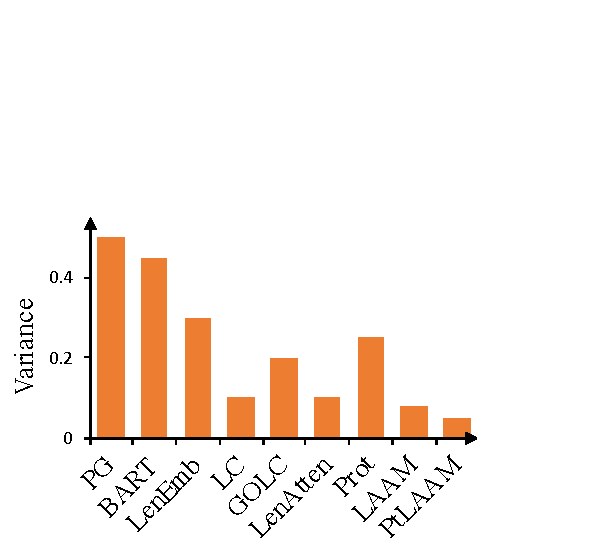
\includegraphics[width=1.58in]{allcnnvar.pdf}
		%\end{minipage}%
	}
	\subfigure[Variance of XSUM]{
	\label{fig:varX}
	%\begin{minipage}[t]{0.5\linewidth}
	\centering
	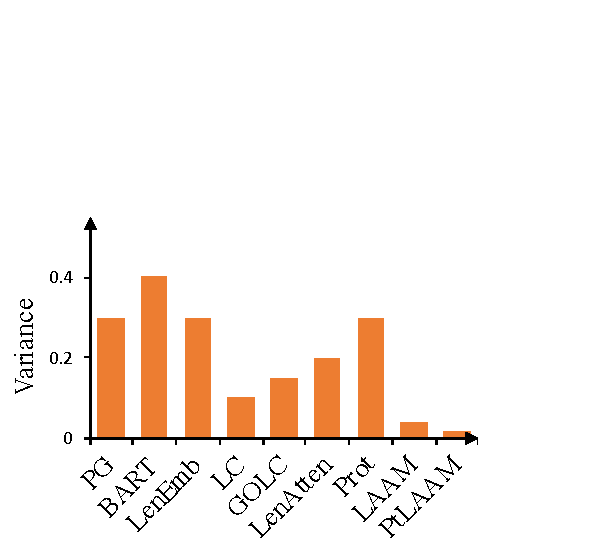
\includegraphics[width=1.58in]{allxvar.pdf}
	%\end{minipage}%
}
	\caption{Variance of summary lengths.}
	\label{fig:var}
\end{figure}


As shown in \tabref{tab:genall}, BART and Prot are the best approaches for non-length-controllable models and length-controllable models respectively.
As shown in \tabref{tab:human}, compared with BART and Prot,
our best approach PtLAAM achieves the best score, which denotes the quality of
summaries generated by PtLAAM is the best.
Prot and PtLAAM preform better than BART, 
which shows the length-controllable approaches
are effective in generating hight-quality summaries.
We also compare BART and Prot with our proposed approaches in the following experiments.

\begin{table}[th]
	\centering
	\scriptsize
	\begin{tabular}{|l|c|c|c|c|}
		\hline 
		& Gold & BART & Prot & PtLAAM\\
		\hline
		CNNDM & \bf{4.2} &  2.4 & 2.6 & 3.4 \\
		XSUM &\bf{4.6} & 2.3 & 2.2 & 2.9 \\
		\hline
	\end{tabular}
	\caption{Human evaluation. Average Cohen's Kappa is 0.62 among judges,
indicating good agreement. 
		%The average pair-wise Kappa coefficient among 3 judges is $0.6$, 
		%indicating substantial agreement.
		%\KZ{How do you compute the kappa coefficient?} 
	}\label{tab:human}  
\end{table}


\textit{Information selection.} 
We apply Exact on the BART, Prote, LAAM and PtLAAM to enforce exact desired length.
As shown in \tabref{tab:exact}, the better performance of our proposed approaches means that 
our approaches can cover more important information under the same length limitation. 
Compared to \tabref{tab:genall} our approaches also show more stability.

\begin{table}[th]
	\centering
	\scriptsize
	\begin{tabular}{|c|m{0.8cm}<{\raggedleft}|c|c|c|c|c|c|}
		\hline
		\multicolumn{2}{|c|}{\multirow{2}{*}{Approach}} & \multicolumn{3}{c|}{\bf CNNDM} &  \multicolumn{3}{c|}{\bf XSUM} \\ \cline{3-8}
		\multicolumn{2}{|c|}{\multirow{2}{*}{}}& R-1 & R-2 & R-L& R-1 & R-2 & R-L \\
		\hline
		\multirow{4}{*}{Exact} & BART 
		            & 43.43& 20.11 & 39.52 & 44.82 & 21.34 & 36.23  \\
     &   Prot & 42.97 & 20.15  & 39.40 &44.81 & 21.53 & 36.42  \\
     &  LAAM & 43.55& 20.21 & 39.75 & 45.08 & 21.77 & 36.64 \\
& PtLAAM & \bf 44.17&\bf 20.38 &\bf 39.97  & \bf 45.48 &\bf 21.80 & \bf 36.84  \\
		\hline
	\end{tabular}
	\caption{Evaluation of models extended with Exact, which fixes
the output length to those of the gold summaries.}\label{tab:exact}  
\end{table}

Besides, as shown in \tabref{tab:exp},
the summaries are generated by the SOTA length-controllable approach Prot and our best approach PtLAAM with desired length as $10$ tokens and $20$ tokens.
For Prot, the summary with desired length as $10$ is just the truncated version of summary with desired length as $20$.
Different from Prot, the content of summaries generated by PtLAAM are changed according to different desired lengths, which shows that PtLAAM is more effective on selecting information to be summarized by length constraint.
\cut{
\begin{table}[th!]
	\centering
	\scriptsize
	\begin{tabular}{|l|p{6cm}|}
		\hline 
		\multicolumn{2}{|c|}{\bf Input Document} \\
		\hline
		\multicolumn{2}{|c|}{ \tabincell{l}{a gym teacher in new hampshire has been accused of posing as a young girl on \\a social media site ...... police charged 34-year-old paul johnson-yarosevich\\ of acton, maine  on monday with prohibited use of computer ......}} \\
		\hline
		\hline 
		\multicolumn{2}{|l|}{\bf Prot Summaries} \\
		\hline 
		\bf  $l=10$ & \textit{police charged 34-year-old paul johnson-yarosevich of acton with prohibited} . \\
		\hline 
		\bf  $l=15$ & \textit{police charged 34-year-old paul johnson-yarosevich of acton}, on monday with prohibited use of computer . \\
		\bf  $l=15$ & \textit{police charged 34-year-old paul johnson-yarosevich of acton}, on monday with prohibited use of computer . \\
		\hline 
		\hline
		\multicolumn{2}{|l|}{\bf PtLAAM Summaries} \\
		\hline 
		\bf  $l=10$ & Paul was prohibited use of computer for cheating . \\
		\hline 
		\bf  $l=15$ & 34-year-old paul johnson-yarosevich has been chart with prohibited use of a computer .                                         
		\\
		\bf  $l=20$ & \textit{police charged 34-year-old paul johnson-yarosevich of acton}, on monday with prohibited use of computer . \\
		\hline 
		
	\end{tabular}
	\caption{Example generated summaries of various desired length. \KZ{Give length 20 as well?}}\label{tab:exp} 
\end{table}
}%%%%
\begin{table}[th!]
	\centering
	\scriptsize
	\begin{tabular}{|p{0.3cm}|p{3cm}|p{3cm}|}
		\hline 
		\multicolumn{3}{|c|}{\bf Input Document} \\
		\hline
		\multicolumn{3}{|c|}{ \tabincell{l}{a gym teacher in new hampshire has been accused of posing as a young girl on \\a social media site ...... police charged 34-year-old paul johnson-yarosevich\\ of acton, maine  on monday with prohibited use of computer ......}} \\
		\hline
		\hline 
         \bf Len & \bf Prot Summaries & \bf PtLAAM Summaries\\
		\hline 
		\bf  $10$ & \tabincell{l}{police charged 34-year-old \\ paul johnson-yarosevich of \\ acton with prohibited .}  & \tabincell{l}{Paul was prohibited use of computer \\ for cheating . } \\
		%\tabincell{l}{\textit{police charged 34-year-old} \\ \textit{paul johnson-yarosevich of} \\ \textit{acton} with prohibited .}  & \tabincell{l}{Paul was prohibited use of computer \\ for cheating . }\\
		\hline 
		\bf  $15$ & \tabincell{l}{\textit{police charged 34-year-old} \\ \textit{paul johnson-yarosevich of} \\ \textit{acton} , on monday with \\ prohibited use of computer . }&
		\tabincell{l}{34-year-old paul johnson-yarosevich \\ has been chart with prohibited use \\ of a computer . }\\
		\hline
		\bf  $20$ & \tabincell{l}{\textit{police charged 34-year-old} \\ \textit{paul johnson-yarosevich of} \\ \textit{acton , on monday with} \\ \textit{prohibited use of computer .} \\ the investigation started \\ in december .}& \tabincell{l}{police charged 34-year-old paul \\  johnson-yarosevich on monday \\with prohibited use of computer after \\ discovering he 'd been fooling a girl .}
		\\
		\hline 
	\end{tabular}
	\caption{Example generated summaries of various desired length \textbf{Len}. \label{tab:exp} The {\em italicized} tokens repeat significant parts
the shorter summaries. }
\end{table}

\begin{figure}[!ht]
	\centering
	\scriptsize
	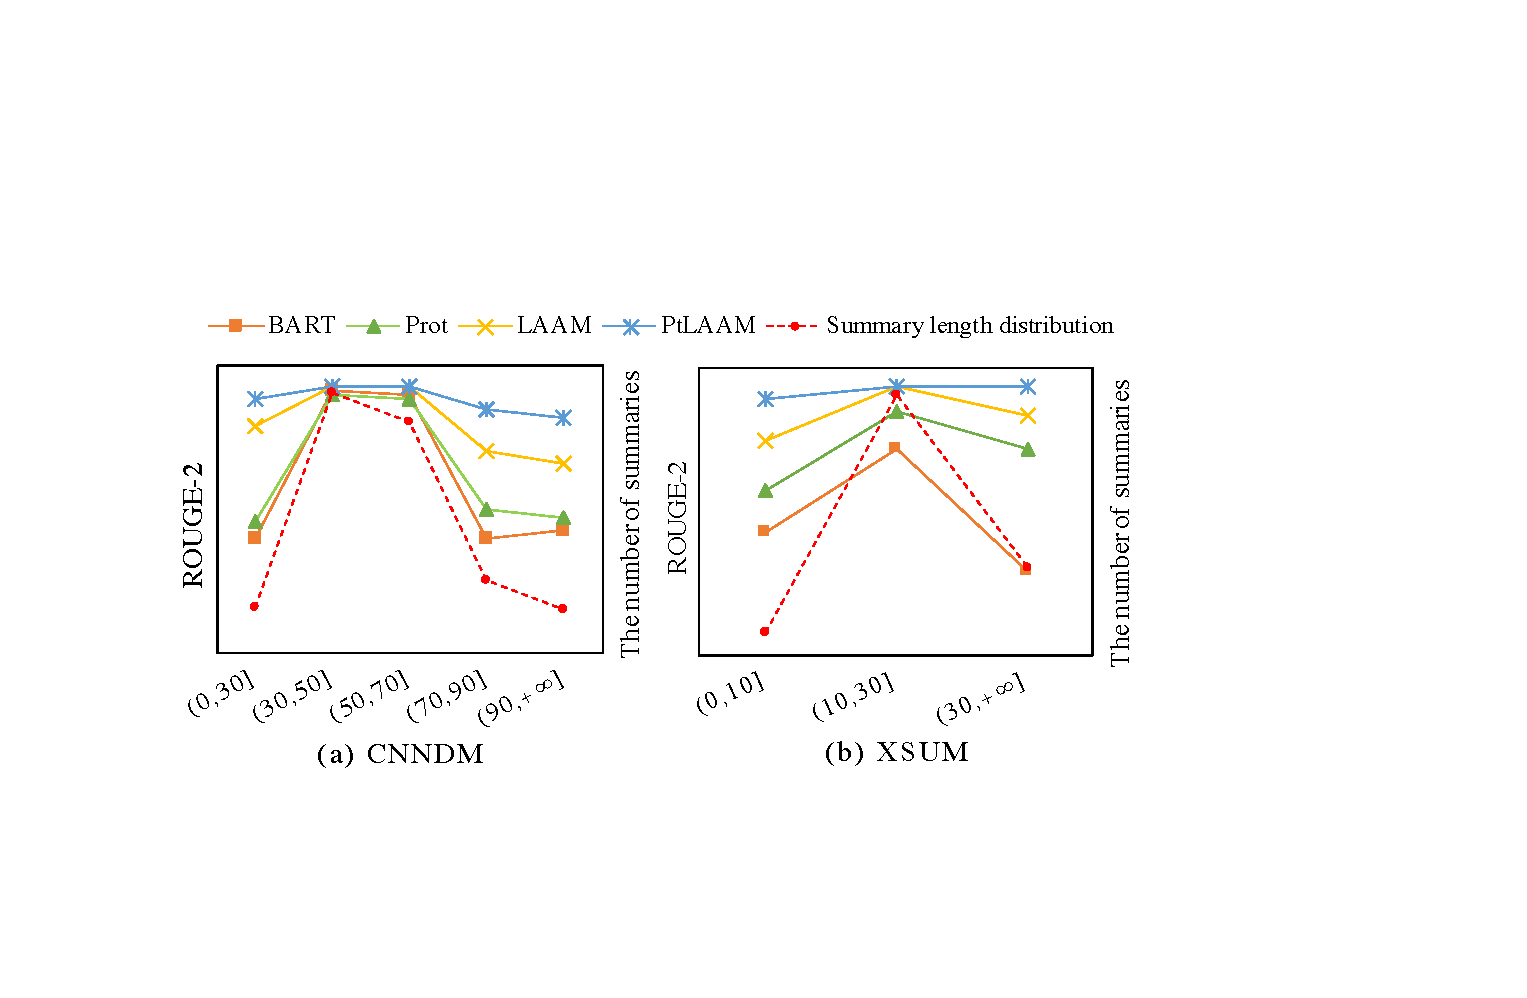
\includegraphics[width=1\linewidth]{rouge.pdf}
	\caption{ROUGE score of models tested by different summary length ranges.}
	\label{fig:rouge}
\end{figure}

\textit{Length control.} To evaluate the effectiveness of controlling length in different length ranges, we divided the test data into different sets according to length range in \tabref{tab:lendis}, and test the models on these sets separately. 
%We take the first length range of CNNDM as $(0,30]$ because the number of summary with length belonging to $(0,10]$ is 1, which cannot be a test set.
As ROUGE-2 is the most popular metric in summarization,
we show the ROUGE-2 scores of models tested on these test sets.
As shown in \figref{fig:rouge},
LAAM and PtLAAM have better ROUGE scores than other methods 
on the test sets in different length ranges.
Meanwhile,
the rouge scores of our approaches on different test sets 
are stable, showing that our approaches are
not affected by the summary length distribution in training set 
and can generate summaries with desired lengths.
%the effectiveness of our approaches on selecting important information to generate high-quality summaries.
As shown in \figref{fig:vars}, the lower variance of LAAM and PtLAAM show the effectiveness of our approach on controlling length.
For the same length range in \tabref{tab:lendis} and \figref{fig:rouge}, the more training data in this range, the lower Var of the generated summaries with respect to the reference summaries within this length range.
This denotes that the imbalance length distribution in trainig data
interferes with controlling length.


\begin{figure}[!ht]
	\centering
	\scriptsize
	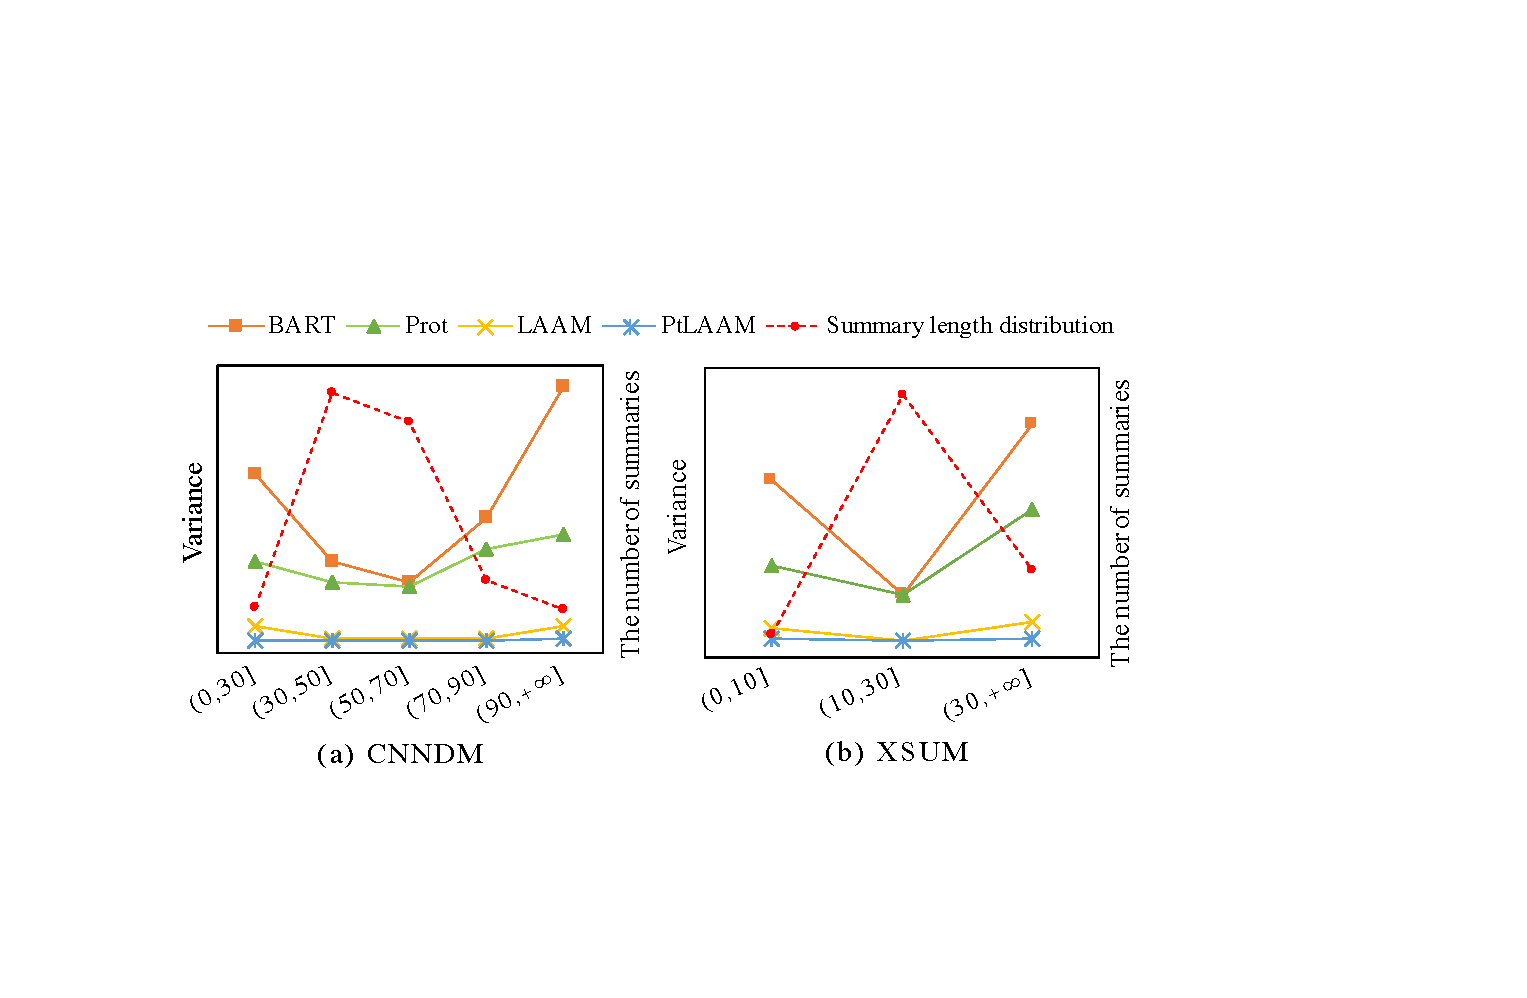
\includegraphics[width=1\linewidth]{vars.pdf}
	\caption{Variance score of models tested by different summary length ranges.}
	\label{fig:vars}
\end{figure}


\cut{%%%%
\begin{table*}[th]
	\scriptsize
	\centering
\subtable[BART]{
	\begin{tabular}{|c|r|ccc|c|}
		\hline
		\bf Data& \bf Length& \bf R-1 & \bf R-2 & \bf R-L &Var \\ 
		\hline
		\multirow{6}{*}{CNNDM} 
		& $(0,30]$ &\bf 33.91& \bf 15.89 &\bf 31.32 & \\
		& $(30,50]$ &  & & & \\
		& $(50,70]$&  &  & &\\
		& $(70,90]$ & & & &\\
		& $(90,+\infty)$ & & & &\\
		\hline
		\multirow{4}{*}{XSUM} 
		&$(0,10]$ & 3,049 & 167 & 176 &\\
		& $(10,30]$ & 193,237 & 10,732 & 10,729 &\\
		& $(30,+\infty)$ & 77,60 & 433 & 429 &\\
		\hline
	\end{tabular}
}
\qquad
\subtable[Prot]{
\begin{tabular}{|c|r|ccc|c|}
	\hline
	\bf Data& \bf Length& \bf R-1 & \bf R-2 & \bf R-L &Var \\ 
	\hline
	\multirow{6}{*}{CNNDM} 
	& $(0,30]$ & 20,429&573 & 487 & \\
	& $(30,50]$ & 114,521 &4,255&4,144& \\
	& $(50,70]$& 101,461 & 4,746 &4,380 &\\
	& $(70,90]$ & 31,470 & 2,321 & 1,509&\\
	& $(90,+\infty)$ & 18,925&1,472 &969 &\\
	\hline
	\multirow{4}{*}{XSUM} 
	&$(0,10]$ & 3,049 & 167 & 176 &\\
	& $(10,30]$ & 193,237 & 10,732 & 10,729 &\\
	& $(30,+\infty)$ & 77,60 & 433 & 429 &\\
	\hline
\end{tabular}
}
\qquad
\subtable[LAAM]{
\begin{tabular}{|c|r|ccc|c|}
	\hline
	\bf Data& \bf Length& \bf R-1 & \bf R-2 & \bf R-L &Var \\ 
	\hline
	\multirow{6}{*}{CNNDM} 
	& $(0,30]$ & 20,429&573 & 487 & \\
	& $(30,50]$ & 114,521 &4,255&4,144& \\
	& $(50,70]$& 101,461 & 4,746 &4,380 &\\
	& $(70,90]$ & 31,470 & 2,321 & 1,509&\\
	& $(90,+\infty)$ & 18,925&1,472 &969 &\\
	\hline
	\multirow{4}{*}{XSUM} 
	&$(0,10]$ & 3,049 & 167 & 176 &\\
	& $(10,30]$ & 193,237 & 10,732 & 10,729 &\\
	& $(30,+\infty)$ & 77,60 & 433 & 429 &\\
	\hline
\end{tabular}
}
\qquad
\subtable[PtLAAM]{
\begin{tabular}{|c|r|ccc|c|}
	\hline
	\bf Data& \bf Length& \bf R-1 & \bf R-2 & \bf R-L &Var \\ 
	\hline
	\multirow{6}{*}{CNNDM} 
	& $(0,30]$ & \bf 33.91& \bf 15.89 &\bf 31.32 & \\
	& $(30,50]$ & 114,521 &4,255&4,144& \\
	& $(50,70]$& 101,461 & 4,746 &4,380 &\\
	& $(70,90]$ & 31,470 & 2,321 & 1,509&\\
	& $(90,+\infty)$ & 18,925&1,472 &969 &\\
	\hline
	\multirow{4}{*}{XSUM} 
	&$(0,10]$ & 3,049 & 167 & 176 &\\
	& $(10,30]$ & 193,237 & 10,732 & 10,729 &\\
	& $(30,+\infty)$ & 77,60 & 433 & 429 &\\
	\hline
\end{tabular}
}
	\caption{Test the models on different summaries with different length ranges. We take the first length as $(0,30]$ because the number of summary with length belonging to $(0,10]$ is 1, which cannot be a test set.
	}\label{tab:genrange}  
\end{table*}

\begin{table*}[th]
	\scriptsize
	\centering
	\begin{tabular}{|c|r|ccc|ccc|ccc|ccc|}
		\hline
		\multirow{2}{*}{\bf Data}& \multirow{2}{*}{\bf Length} & \multicolumn{3}{|c|}{\bf BART} &  \multicolumn{3}{|c|}{\bf Prot} & \multicolumn{3}{|c|}{\bf LAAM} & \multicolumn{3}{|c|}{\bf PtLAAM} \\
		\cline{3-14}
		& & \bf R-1 & \bf R-2 & \bf R-L & \bf R-1 & \bf R-2 & \bf R-L& \bf R-1 & \bf R-2 & \bf R-L& \bf R-1 & \bf R-2 & \bf R-L \\ 
		\hline
		\multirow{6}{*}{CNNDM} 
		& $(0,30]$ & \bf 33.91& \bf 15.89 &\bf 31.32 & & & & & & & & & \\
		& $(30,50]$ & 114,521 &4,255&4,144& & & & & & & & & \\
		& $(50,70]$& 101,461 & 4,746 &4,380 & & & & & & & & & \\
		& $(70,90]$ & 31,470 & 2,321 & 1,509& & & & & & & & &\\
		& $(90,+\infty)$ & 18,925&1,472 &969 & & & & & & & & \\
		\hline
		\multirow{4}{*}{XSUM} 
		&$(0,10]$ & 3,049 & 167 & 176 & & & & & & & & \\
		& $(10,30]$ & 193,237 & 10,732 & 10,729 && & & & & & & &\\
		& $(30,+\infty)$ & 77,60 & 433 & 429 & & & & & & & & &\\
		\hline
	\end{tabular}
\caption{Test the models on different summaries with different length ranges. We take the first length as $(0,30]$ because the number of summary with length belonging to $(0,10]$ is 1, which cannot be a test set.
}\label{tab:genrange}  
\end{table*}
}%%%%%

\subsubsection{Ablation Studies}
We evaluate the effectiveness of the pretraining LAAM on LBD,
and the effectiveness of length-aware attention mechanism.

\textit{Pretraining using LBD.} 
As shown in \figref{fig:rouge} and \figref{fig:vars},
compared with LAAM only training on original datasets, PtLAAM performs better on ROUGE and Var. 
The better ROUGE scores in \figref{fig:rouge} show that the PtLAAM can select more important information with pretrained LAAM on our created dataset LBD.
As one source document of LBD may have different extracted summaries within different length ranges, the model trained on LBD can learn to select different information from source document according to the length constraints.
Besides, in LBD, the number of summaries with length in different ranges is balanced.
As shown in \figref{fig:vars},
PtLAAM gets lower Var, which shows it can controlling length better.
The Vars in different length ranges are stable, which 
weakens the negative impact caused by the imbalanced length distribution of training data. 

\textit{Length-aware attention mechanism,}
The length-aware attention consists of $Attn_{is}$ and $Attn_{eos}$.
As shown in \tabref{tab:lenattn},
compared with LAAM, 
the LAAM without $Attn_{is}$ in length-aware attention has a big drop in ROUGE scores
and a small drop in Var score,
which shows that $Attn_{is}$ mainly focuses on select information with length constraint.
The LAAM without $Attn_{eos}$ gets the much lower Var scores and less lower ROUGE scores than LAAM,
which denotes that $Attn_{eos}$ is useful in limiting the output length.
LAAM outperforms its variant because of the effectiveness of length-aware attention mechanism. Thus, in our experiments, 
we use PtLAAM model, which trains LAAM with both $Attn_{is}$ and $Attn_{eos}$
on LBD first and then fine-tunes the original datasets, as our best approaches.

\begin{table}[th]
	\centering
	\scriptsize
	\begin{tabular}{|c|lc|c|c|c|c|}
		\hline 
		Data & \multicolumn{2}{c|}{Model} & R-1 & R-2&R-L&Var (\%)\\
		\hline
		\multirow{3}{*}{CNNDM} & \multicolumn{2}{l|}{LAAM} & \bf 43.55& \bf 20.20 & \bf 39.73 &\bf 0.05  \\ 
		&&w/o $Attn_{is}$ & 42.77 &  19.32 & 39.13 & 0.06\\
		&&w/o $Attn_{eos}$ & 43.10 &  20.17 & 37.45 & 0.13\\
		\hline
		\multirow{3}{*}{XSUM} &\multicolumn{2}{l|}{LAAM} & \bf 45.00 & \bf 21.77 & \bf 36.64 & \bf 0.03 \\ 
		&&w/o $Attn_{is}$ & 43.45 & 20.64 & 34.79 & 0.03 \\
		&&w/o $Attn_{eos}$ & 44.62 &  21.32 & 35.03 & 0.08\\
		\hline
	\end{tabular}
	\caption{Usefulness of two kinds of attentions.} 
	\label{tab:lenattn}  
\end{table}

\subsection{Experiment 2: Zero-shot Length Control}
\label{sec:zeroshot}
In this experiment, zero-shot task is to generate summaries within a short length range by a model trained on dataset removing summaries within the same length range. We use the modified dataset for zero-shot length control.
The performance of length-controllable approaches on zero-shot task can evaluate the effectiveness of them in controlling output length.

As shown in \tabref{tab:zero}, the performance of PtLAAM on ROUGE scores and Var on different datatsets are the best.
The ROUGE scores are similar in \tabref{tab:zero}.
The reason is that 
the lengths of summaries generated by BART and Prot 
are longer than the reference summaries, which results in the generated summaries may match more tokens in reference.
We use F1 scores to evaluate the generated summaries, which penalizes the summaries with longer length. 
Thus, compared with PtLAAM, 
the ROUGE scores of other approaches in \tabref{tab:zero} are similar but smaller than PtLAAM.
The lowest Var of our proposed models shows that our approach can 
better control length in seq2seq summarization model.
The LAAM gets higher Var and lower ROUGE scores than PtLAAM denotes that
the ability of LAAM to control length are impacted by length distribution of the training data.
This also shows that the pretraining on LBD in PtLAAM is useful in generating high-quality summaries under desired summary length since the distribution of summaries in different length ranges are balance in LBD.

\begin{table}[th]
	\scriptsize
	\centering
		\begin{tabular}{|c|c|r|ccc|c|}
			\hline
			\bf Dataset& \bf Length &\bf Approach& \bf R-1 & \bf R-2 & \bf R-L &Var (\%) \\ 
			\hline
			\multirow{4}{*}{CNNDM} 
			& \multirow{4}{*}{$(0,30]$}  & BART & 32.27 &14.40 & 28.66 & 0.40 \\
			&& Prot & 33.04 &14.83& 29.42 & 0.14 \\
			&& LAAM & 33.64 & 15.23 & 30.76 & 0.05 \\
			&& PtLAAM & \bf 33.78& \bf 15.89 &\bf 31.30 & \bf 0.03\\
			\hline
			\multirow{4}{*}{XSUM} 
		& \multirow{4}{*}{$(0,10]$} & BART & 33.97&19.12& 31.28 & 0.28\\
	&& Prot & 34.37 & 19.54 & 31.66 & 0.10 \\
	&& LAAM & 34.83 &  20.15&32.10 & 0.03\\
	&& PtLAAM & \bf 35.16& \bf 20.58 & \bf 32.49 & \bf 0.02\\
			\hline
		\end{tabular}
	\caption{Results of zero-shot length control. The length 
refers to length of reference summaries in test set.}\label{tab:zero}  
\end{table}

